\documentclass[12pt,addpoints]{exam}

\newcommand{\class}{10-423/10-623 Gen AI}
\newcommand{\term}{Fall 2024}
\newcommand{\examnum}{Quiz 2}
\newcommand{\examdate}{09/30/24}
\newcommand{\timelimit}{15 minutes} % This one was 18-20 minutes in S24
%% To HIDE SOLUTIONS, set this value to 0: 
% \providecommand{\issoln}{0}
\providecommand{\issoln}{1}

%-----------------------------------------------------------------------------
% PACKAGES AND OTHER DOCUMENT CONFIGURATIONS
%-----------------------------------------------------------------------------

\usepackage[margin=1in]{geometry}
\usepackage{amsmath, amsfonts}
\usepackage{enumerate}
\usepackage{graphicx}
\usepackage{titling}
\usepackage{url}
\usepackage{xfrac}
\usepackage{natbib}
\usepackage{amssymb}
\usepackage{amsthm}
\usepackage{paralist}
\usepackage{epstopdf}
\usepackage{tabularx}
\usepackage{longtable}
\usepackage{multirow}
\usepackage{multicol}
\usepackage[colorlinks=true,urlcolor=blue]{hyperref}
\usepackage{algorithm}
\usepackage{algorithmicx}
\usepackage[noend]{algpseudocode}
\usepackage{float}
\usepackage{enumerate}
\usepackage{array}
\usepackage{environ}
\usepackage{times}
\usepackage{textcomp}
\usepackage{caption}
\usepackage{parskip} % For NIPS style paragraphs.
\usepackage[compact]{titlesec} % Less whitespace around titles
\usepackage[inline]{enumitem} % For inline enumerate* and itemize*
\usepackage{datetime}
\usepackage{comment}
% \usepackage{minted}
\usepackage{lastpage}
\usepackage{color}
% \usepackage{xcolor}
\usepackage[dvipsnames]{xcolor}
\usepackage[final]{listings}
\usepackage{tikz}
\usetikzlibrary{shapes,decorations}
\usepackage{framed}
\usepackage{booktabs}
\usepackage{cprotect}
\usepackage{verbatimbox}
\usepackage{multicol}
\usepackage{hyperref}
\usepackage{subcaption}
\usepackage{mathtools} % For drcases
\usepackage{cancel}
\usepackage[many]{tcolorbox}
\tcbuselibrary{listings} % For listings within tcolorbox
\usepackage{soul}
\usepackage[bottom]{footmisc}
\usepackage{bm}
\usepackage{wasysym}
\usepackage{lipsum}

\usepackage{tikz}
\usetikzlibrary{arrows}
\usetikzlibrary{arrows.meta}
\usetikzlibrary{shapes.geometric}
\usetikzlibrary{positioning, arrows, automata, calc}
\usepackage{transparent}
\usepackage{tikz-cd}

%%%%%%%%%%%%%%%%%%%%%%%%%%%%%%%%%%%%%%%%%%%
% Formatting for \CorrectChoice of "exam" %
%%%%%%%%%%%%%%%%%%%%%%%%%%%%%%%%%%%%%%%%%%%

\CorrectChoiceEmphasis{}
\checkedchar{\blackcircle}

\newenvironment{checkboxessquare}{
    \begingroup
    \checkboxchar{$\Box$} \checkedchar{$\blacksquare$} % change checkbox style locally
    \begin{checkboxes}
    }{
    \end{checkboxes}
    \endgroup
    }

    
\newenvironment{oneparcheckboxessquare}{
    \begingroup
    \checkboxchar{$\Box$} \checkedchar{$\blacksquare$} % change checkbox style locally
    \begin{oneparcheckboxes}
    }{
    \end{oneparcheckboxes}
    \endgroup
    }

%%%%%%%%%%%%%%%%%%%%%%%%%%%%%%%%%%%%%%%%%%%
% Better numbering                        %
%%%%%%%%%%%%%%%%%%%%%%%%%%%%%%%%%%%%%%%%%%%

% \numberwithin{equation}{section} % Number equations within sections (i.e. 1.1, 1.2, 2.1, 2.2 instead of 1, 2, 3, 4)
% \numberwithin{figure}{section} % Number figures within sections (i.e. 1.1, 1.2, 2.1, 2.2 instead of 1, 2, 3, 4)
% \numberwithin{table}{section} % Number tables within sections (i.e. 1.1, 1.2, 2.1, 2.2 instead of 1, 2, 3, 4)

%%%%%%%%%%%%%%%%%%%%%%%%%%%%%%%%%%%%%%%%%%
% Custom commands                        %
%%%%%%%%%%%%%%%%%%%%%%%%%%%%%%%%%%%%%%%%%%
\newcommand{\blackcircle}{\tikz\draw[black,fill=black] (0,0) circle (1ex);}
\renewcommand{\circle}{\tikz\draw[black] (0,0) circle (1ex);}

\newcommand{\solo}{ \textcolor{orange}{[SOLO]} }
\newcommand{\open}{ \textcolor{blue}{[OPEN]} }

\input{../shared/mathabbreviations.tex}

%%%%%%%%%%%%%%%%%%%%%%%%%%%%%%%%%%%%%%%%%%%
% Code highlighting with listings         %
%%%%%%%%%%%%%%%%%%%%%%%%%%%%%%%%%%%%%%%%%%%

\definecolor{bluekeywords}{rgb}{0.13,0.13,1}
\definecolor{greencomments}{rgb}{0,0.5,0}
\definecolor{redstrings}{rgb}{0.9,0,0}
\definecolor{light-gray}{gray}{0.95}

\newcommand{\MYhref}[3][blue]{\href{#2}{\color{#1}{#3}}}%

\definecolor{dkgreen}{rgb}{0,0.6,0}
\definecolor{gray}{rgb}{0.5,0.5,0.5}
\definecolor{mauve}{rgb}{0.58,0,0.82}

\lstdefinelanguage{Shell}{
  keywords={tar, cd, make},
  %keywordstyle=\color{bluekeywords}\bfseries,
  alsoletter={+},
  ndkeywords={python3, python, py, javac, java, gcc, c, g++, cpp, .txt, octave, m, .tar},
  %ndkeywordstyle=\color{bluekeywords}\bfseries,
  identifierstyle=\color{black},
  sensitive=false,
  comment=[l]{//},
  morecomment=[s]{/*}{*/},
  commentstyle=\color{purple}\ttfamily,
  %stringstyle=\color{red}\ttfamily,
  morestring=[b]',
  morestring=[b]",
  backgroundcolor = \color{light-gray}
}

\lstset{columns=fixed, basicstyle=\ttfamily,
    backgroundcolor=\color{light-gray},xleftmargin=0.5cm,frame=tlbr,framesep=4pt,framerule=0pt}

\newcommand{\emptysquare}{{\LARGE $\square$}\ \ }
\newcommand{\filledsquare}{{\LARGE $\boxtimes$}\ \ }
\def \ifempty#1{\def\temp{#1} \ifx\temp\empty }


% \newcommand{\squaresolutionspace}[2][\emptysquare]{\newline #1}{#2}
\def \squaresolutionspace#1{ \ifempty{#1} \emptysquare \else #1\hspace{0.75pt}\fi}
\newcommand{\squaresoln}[0]{ \begin{soln}\filledsquare \end{soln}}


\newcommand{\emptycircle}{{\LARGE $\fullmoon$}\ \ }
\newcommand{\filledcircle}{{\LARGE $\newmoon$}\ \ }
\def \circlesolutionspace#1{ \ifempty{#1} \emptycircle \else #1\hspace{0.75pt}\fi}
\newcommand{\circlesoln}[0]{ \begin{soln}\filledcircle \end{soln}}
%%%%%%%%%%%%%%%%%%%%%%%%%%%%%%%%%%%%%%%%%%%
% Custom box for highlights               %
%%%%%%%%%%%%%%%%%%%%%%%%%%%%%%%%%%%%%%%%%%%

% Define box and box title style
\tikzstyle{mybox} = [fill=blue!10, very thick,
    rectangle, rounded corners, inner sep=1em, inner ysep=1em]

% \newcommand{\notebox}[1]{
% \begin{tikzpicture}
% \node [mybox] (box){%
%     \begin{minipage}{\textwidth}
%     #1
%     \end{minipage}
% };
% \end{tikzpicture}%
% }

\NewEnviron{notebox}{
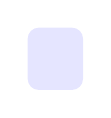
\begin{tikzpicture}
\node [mybox] (box){
    \begin{minipage}{0.95\textwidth}
        \BODY
    \end{minipage}
};
\end{tikzpicture}
}

%%%%%%%%%%%%%%%%%%%%%%%%%%%%%%%%%%%%%%%%%%%
% Commands showing / hiding solutions     %
%%%%%%%%%%%%%%%%%%%%%%%%%%%%%%%%%%%%%%%%%%%
\newcommand{\solutionspace}[4]{\fbox{\begin{minipage}[t][#1][t]{#2} \textbf{#3} \solution{}{#4} \end{minipage}}}

% To HIDE SOLUTIONS, set this value to 0:
%\providecommand{\issoln}{0}
%\providecommand{\issoln}{1}

\ifthenelse{\equal{\issoln}{1}}{

% SOLUTION environment
\newenvironment{soln}{\leavevmode\color{red}\ignorespaces }{}

% QUESTION AUTHORS environment
\newenvironment{qauthor}{\leavevmode\color{blue}\ignorespaces }{}

% Question tester comment environment
\newenvironment{qtester}{\leavevmode\color{green}\ignorespaces}{}

% Question learning objective comment environment
\newenvironment{qlearningobjective}{\leavevmode\color{green}\ignorespaces}{}

}{ % ELSE

  \NewEnviron{soln}{}
  \NewEnviron{qauthor}{}
  \NewEnviron{qtester}{}
  \NewEnviron{qlearningobjective}{}

}

%% To HIDE TAGS set this value to 0:
\def\showtags{0}
%%%%%%%%%%%%%%%%
\ifcsname showtags\endcsname \else \def\showtags{1} \fi
% Default to an empty tags environ.
\NewEnviron{tags}{}{}
\if\showtags 1
% Otherwise, include solutions as below.
\RenewEnviron{tags}{
    \fbox{
    \leavevmode\color{blue}\ignorespaces
    \textbf{TAGS:} \texttt{\url{\BODY}}
    }
    \vspace{-.5em}
}{}
\fi

\newtcolorbox[]{answer_box}[1][]
{
    % breakable,
    fit,
    enhanced,
    % nobeforeafter,
    colback=white,
    title=Your Answer,
    sidebyside align=top,
    box align=top,
    #1
}

% This must be specified with option brackets \begin{answerboxcode}[] \end{answerboxcode}
% For some reason, this would break if we used the name answer_box_code
\newtcblisting{answerboxcode}[1][]
{
    listing only,
    listing options={
        language=Python,
        showstringspaces=false,     % Don't show spaces in strings
        tabsize=4,                  % Set tab size to 4 spaces
        breaklines=true,            % Break long lines
        numbers=left,               % Line numbers on the left
    },
    height=6cm,
    width=15cm,
    fit,
    enhanced,
    colback=white,
    title=Your Answer,
    sidebyside align=top,
    box align=top,
    #1
}

%\pagestyle{fancyplain}
\lhead{\hwName{}
\begin{soln}Solutions\end{soln}
}
\rhead{\courseNum}
\cfoot{\thepage{} of \numpages{}}

\title{\textsc{\hwNum}
\begin{soln}Solutions\end{soln}
\\
\textsc{\hwTopic}
\thanks{Compiled on \today{} at \currenttime{}}\\
\vspace{1em}
} % Title


\author{\textsc{\large \courseNum{} \courseName{}}\\
\courseUrl
\vspace{1em}\\
\ifdefempty{\outDate}{}{  OUT: \outDate \\ }
\ifdefempty{\dueDate}{}{  DUE: \dueDate \\ }
\ifdefempty{\taNames}{}{  TAs: \taNames{} }
}

\date{}

%%%%%%%%%%%%%%%%%%%%%%%%%%%%%%%%%%%%%%%%%%%%%%%%%
% Useful commands for typesetting the questions %
%%%%%%%%%%%%%%%%%%%%%%%%%%%%%%%%%%%%%%%%%%%%%%%%%

% This command will allow long \lstinline{} text to wrap automatically.
\sloppy

%%%%%%%%%%%%%%%%%%%%%%%%%%
% Document configuration %
%%%%%%%%%%%%%%%%%%%%%%%%%%

% Don't display a date in the title and remove the white space
\predate{}
\postdate{}
\date{}

% Don't display an author and remove the white space
% \preauthor{}
% \postauthor{}

% Question type commands
\newcommand{\sall}{\textbf{Select all that apply: }}
\newcommand{\sone}{\textbf{Select one: }}
\newcommand{\tf}{\textbf{True or False: }}




% Changes to examdoc
\qformat{\textbf{{\Large \thequestion \; \; \thequestiontitle \ (\totalpoints \ points)}} \hfill}
\renewcommand{\thequestion}{\arabic{question}}
\renewcommand{\questionlabel}{\thequestion.}

\renewcommand{\thepartno}{\thequestion.\arabic{partno}}
%\renewcommand{\partlabel}{\thequestion.\thepartno.}
\renewcommand{\partlabel}{\thepartno.}

% not working: \renewcommand{\subpartlabel}{(\thequestion.\thepartno.\thesubpart)}
% Commented after adding \question.\thepartno.
%\renewcommand{\partshook}{\setlength{\leftmargin}{0pt}}

\renewcommand{\thesubpart}{\thepartno.\alph{subpart}}
\renewcommand{\subpartlabel}{\thesubpart.}

\renewcommand{\thesubsubpart}{\thesubpart.\roman{subsubpart}}
\renewcommand{\subsubpartlabel}{\thesubsubpart.}

% copied from stack overflow, as all good things are
\newcommand\invisiblesection[1]{%
  \refstepcounter{section}%
  \addcontentsline{toc}{section}{\protect\numberline{\thesection}#1}%
  \sectionmark{#1}}

% quite possibly the worst workaround i have made for this class
\newcommand{\sectionquestion}[1]{
\titledquestion{#1}
\invisiblesection{#1}
~\vspace{-1em}
}

%%%%%%%%%%%%%%%%%%%%%%%%%%%%%%%%%%%%%%%%%%%
% New Environment for Pseudocode          %
%%%%%%%%%%%%%%%%%%%%%%%%%%%%%%%%%%%%%%%%%%%

% Python style for highlighting
\DeclareFixedFont{\ttb}{T1}{txtt}{bx}{n}{12} % for bold
\DeclareFixedFont{\ttm}{T1}{txtt}{m}{n}{12}  % for normal

\definecolor{deepblue}{rgb}{0,0,0.5}
\definecolor{deepred}{rgb}{0.6,0,0}
\definecolor{deepgreen}{rgb}{0,0.5,0}

\newcommand\pythonstyle{\lstset{
language=Python,
basicstyle=\ttm,
morekeywords={self},              % Add keywords here
keywordstyle=\ttb\color{deepblue},
emph={MyClass,__init__},          % Custom highlighting
emphstyle=\ttb\color{deepred},    % Custom highlighting style
stringstyle=\color{deepgreen},
frame=tb,                         % Any extra options here
showstringspaces=false
}}


% Python environment
\lstnewenvironment{your_code_solution}[1][]
{
\pythonstyle
\lstset{#1}
}
{}


\begin{document}

\section*{Instructions for Specific Problem Types}

For ``Select One" questions, please fill in the appropriate bubble completely:

\begin{quote}
\textbf{Select One:} Who taught this course?
    \begin{list}{}
     \item\CIRCLE{} Matt Gormley
     \item\Circle{} Marie Curie
     \item\Circle{} Noam Chomsky
    \end{list}
\end{quote}

If you need to change your answer, you may cross out the previous answer and bubble in the new answer:

\begin{quote}
\textbf{Select One:} Who taught this course?
    \begin{list}{}
     \item\CIRCLE{} Henry Chai
     \item\Circle{} Marie Curie \\[0.25cm]
     \xcancel{\CIRCLE}{} Noam Chomsky
    \end{list}
\end{quote}

For ``Select all that apply" questions, please fill in all appropriate squares completely:

\begin{quote}
\textbf{Select all that apply:} Which are instructors for this course?
    \begin{list}{}
    \item $\blacksquare$ Matt Gormley  
    \item $\blacksquare$ Henry Chai
    \item $\blacksquare$  Hoda Heidari
    \item $\square$ I don't know
    \end{list}
\end{quote}

Again, if you need to change your answer, you may cross out the previous answer(s) and bubble in the new answer(s):

\begin{quote}
\textbf{Select all that apply:} Which are the instructors for this course?
    \begin{list}{}
    \item $\blacksquare$ Matt Gormley 
    \item $\blacksquare$ Henry Chai
    \item $\blacksquare$ Hoda Heidari \\[0.25cm]
    \xcancel{$\blacksquare$} I don't know
    \end{list}
\end{quote}

For questions where you must fill in a blank, please make sure your final answer is fully included in the given space. You may cross out answers or parts of answers, but the final answer must still be within the given space.

\begin{quote}
\textbf{Fill in the blank:} What is the course number?

\begin{tcolorbox}[fit,height=1cm, width=4cm, blank, borderline={1pt}{-2pt},nobeforeafter]
    \begin{center}\huge10-601\end{center}
    \end{tcolorbox}\hspace{2cm}
    \begin{tcolorbox}[fit,height=1cm, width=4cm, blank, borderline={1pt}{-2pt},nobeforeafter]
    \begin{center}\huge10-\xcancel{6}301\end{center}
    \end{tcolorbox}
\end{quote}


% \section*{Instructions for Specific Problem Types}

For ``Select One" questions, please fill in the appropriate bubble completely:

\begin{quote}
\textbf{Select One:} Who taught this course?
    \begin{checkboxes}
     \CorrectChoice Matt Gormley
     \choice Marie Curie
     \choice Noam Chomsky
    \end{checkboxes}
\end{quote}

If you need to change your answer, you may cross out the previous answer and bubble in the new answer:

\begin{quote}
\textbf{Select One:} Who taught this course?
    {
    \begin{checkboxes}
     \CorrectChoice Henry Chai
     \choice Marie Curie \checkboxchar{\xcancel{\blackcircle}{}}
     \choice Noam Chomsky
    \end{checkboxes}
    }
\end{quote}

For ``Select all that apply" questions, please fill in all appropriate squares completely:

\begin{quote}
\textbf{Select all that apply:} Which are scientists?
    \begin{checkboxessquare}
    \CorrectChoice Stephen Hawking 
    \CorrectChoice Albert Einstein
    \CorrectChoice Isaac Newton
    \choice I don't know
    \end{checkboxessquare}
\end{quote}

Again, if you need to change your answer, you may cross out the previous answer(s) and bubble in the new answer(s):

\begin{quote}
\textbf{Select all that apply:} Which are scientists?
    \begin{checkboxessquare}
    \CorrectChoice Stephen Hawking 
    \CorrectChoice Albert Einstein
    \CorrectChoice Isaac Newton
    \choice I don't know
    \end{checkboxessquare}
\end{quote}

For questions where you must fill in a blank, please make sure your final answer is fully included in the given space. You may cross out answers or parts of answers, but the final answer must still be within the given space.

\begin{quote}
\textbf{Fill in the blank:} What is the course number?

\begin{tcolorbox}[fit,height=1cm, width=4cm, blank, borderline={1pt}{-2pt},nobeforeafter]
    \begin{center}\huge10-425\end{center}
    \end{tcolorbox}\hspace{2cm}
    \begin{tcolorbox}[fit,height=1cm, width=4cm, blank, borderline={1pt}{-2pt},nobeforeafter]
    \begin{center}\huge10-\xcancel{4}625\end{center}
    \end{tcolorbox}
\end{quote}

% \clearpage

\begin{questions}

\sectionquestion{Deep Models for Vision}
\begin{parts}

\part[2] \textbf{Select all that apply:} Suppose you are training a CNN and you are concerned that the dimensionality of your first convolutional layer's output is too large. Which of the following changes to your model's architecture would cause the first convolutional layer's output dimensionality to \emph{decrease}?
\begin{checkboxessquare}
     \choice Increasing the stride in this layer
     \choice Increasing the padding around the input to this layer
     \choice Increasing the dimensionality of the input to this layer
     \choice Increasing the filter size in this layer
     \choice None of the above
\end{checkboxessquare}
\begin{soln}
    A, D
\end{soln}
\begin{qauthor} 
    Henry
\end{qauthor}

\part[1] \textbf{True or False:} The primary difference between a decoder-only transformer and an encoder-only transformer is that a token in a decoder-only transformer cannot attend to tokens that come \emph{after} it in the input sequence whereas a token in an encoder-only transformer cannot attend to tokens that come \emph{before} it in the input sequence. 
\begin{checkboxes}
    \choice True 
    \choice False
\end{checkboxes}
\begin{soln}
    False
\end{soln}
\begin{qauthor}
    Henry
\end{qauthor}

\begin{comment}
\part[1] \textbf{Select one:} What component of an image does a vision transformer use as the \emph{tokens} when constructing an input sequence? 
\begin{checkboxes}
    \choice RGB channels
    \choice Relevant macro-features 
    \choice Fixed-size patches
    \choice Individual pixels
\end{checkboxes}
\begin{soln}
    C
\end{soln}
\begin{qauthor}
    Henry
\end{qauthor}
\end{comment}

\end{parts}

\clearpage
\sectionquestion{GANs}
\begin{parts}

\part[1] \textbf{True or False:} In a generative adversarial network, both the discriminator and the generator must be convolutional neural networks. 
\begin{checkboxes}
    \choice True 
    \choice False
\end{checkboxes}
\begin{soln}
    False
\end{soln}
\begin{qauthor}
    Henry
\end{qauthor}

\part[1] \textbf{Select one:} Which of the following statements best describes how the hyperparameter $k$ is used in the training of a GAN?
\begin{checkboxes}
    \choice The discriminator is trained to convergence $k$ times, each time using a different random initialization. Then the discriminator with the lowest loss is used to train the generator to convergence. 
    \choice The generator is trained to convergence $k$ times, each time using a different random initialization. Then the generator with the lowest loss is used to train the discriminator to convergence. 
    \choice The discriminator \emph{and} the generator are trained simultaneously for $k$ steps of mini-batch SGD. Then, keeping the discriminator fixed, the generator is trained for one step of mini-batch SGD. 
    \choice The discriminator is trained for $k$ steps of mini-batch SGD while keeping the generator fixed. Then, keeping the discriminator fixed, the generator is trained for one step of mini-batch SGD. 
\end{checkboxes}
\begin{soln}
    D
\end{soln}
\begin{qauthor}
    Henry
\end{qauthor}
\end{parts}

\clearpage
\sectionquestion{VAEs}
\begin{parts}

\part[2] \textbf{Select all that apply:} Which of the following statements about the KL divergence term in the VAE objective function \emph{as presented in Lecture 6} is/are true?
\begin{checkboxessquare}
     \choice The arguments of the KL divergence are the decoder's learned distribution over images and a prior distribution over images in the training dataset. 
     \choice The KL divergence term is meant to encourage the encoder to learn a dense distribution over the latent space.
     \choice A common choice for the prior distribution is a uniform distribution over the unit hypercube.
     \choice The KL divergence term acts as a regularizer and can prevent the model from overfitting to the empirical distribution of images in the training dataset.
     \choice None of the above
\end{checkboxessquare}
\begin{soln}
    B, D
\end{soln}
\begin{qauthor} 
    Henry
\end{qauthor}

\part[1] \textbf{Select one:} Which equation below represents how a VAE uses the \emph{reparameterization trick} to model the random variable $\mathbf{z} \sim \mathcal{N}(\boldsymbol\mu_{\boldsymbol\theta}, \boldsymbol\sigma^2_{\boldsymbol\theta})$?
\begin{checkboxes}
    \choice $z = \boldsymbol\mu_{\boldsymbol\theta} + \boldsymbol\epsilon$ where $\boldsymbol\epsilon \sim \mathcal{N}(\mathbf{0}, \boldsymbol\sigma^2_{\boldsymbol\theta})$
    \choice $z = \boldsymbol\sigma_{\boldsymbol\theta}^T\boldsymbol\epsilon$ where $\boldsymbol\epsilon \sim \mathcal{N}(\boldsymbol\mu_{\boldsymbol\theta}, I)$
    \choice $z = \boldsymbol\sigma_{\boldsymbol\theta} \odot \boldsymbol\epsilon$ where $\boldsymbol\epsilon \sim \mathcal{N}(\boldsymbol\mu_{\boldsymbol\theta}, I)$
    \choice $z = \boldsymbol\mu_{\boldsymbol\theta} + \boldsymbol\sigma_{\boldsymbol\theta}^T\boldsymbol\epsilon$ where $\boldsymbol\epsilon \sim \mathcal{N}(\mathbf{0}, I)$
    \choice $z = \boldsymbol\mu_{\boldsymbol\theta} + \boldsymbol\sigma_{\boldsymbol\theta} \odot \boldsymbol\epsilon$ where $\boldsymbol\epsilon \sim \mathcal{N}(\mathbf{0}, I)$
\end{checkboxes}
\begin{soln}
    E
\end{soln}
\begin{qauthor}
    Henry
\end{qauthor}

\part[1] \textbf{True or False:} In a VAE, the variational approximation is also called a ``decoder'' and gives a distribution over images $\xv$ conditioned on a latent $\zv$. 
    \begin{checkboxes}
     \choice True 
     \choice False
    \end{checkboxes}
    \begin{soln}
    Input solution here.
    \end{soln}
    \begin{qauthor}
    False, the decoder $p_{\phi}(\xv \mid \zv)$ is part of the model $p_{\phi}(\xv, \zv)$ we wish to approximate, the encoder $q_{\theta}(\zv \mid \xv)$ is the variational approximation to the model's posterior $p_{\phi}(\zv \mid \xv)$. 
    \end{qauthor}

\end{parts}

\clearpage
\sectionquestion{Diffusion Models}
\begin{parts}

\part[2] \textbf{Select all that apply:} Which of the following are valid statements about the \emph{exact} reverse process $q_{\phi}(\xv_T) \prod_{t=1}^T q_{\phi}(\xv_{t-1} \mid \xv_t)$ in a Denoising Diffusion Probabilistic Model (DDPM)?
    \begin{checkboxessquare}
     \choice $q_{\phi}(\xv_{t-1} \mid \xv_t)$ can be computed efficiently in closed form because it is a product of Gaussian densities
     \choice $q_{\phi}(\xv_{t-1} \mid \xv_t)$ cannot be computed efficiently because of its dependence on $q(\xv_0)$
     \choice The parameters $\phi$ of the exact reverse process are learned from unlabeled training images
     \choice The parameters $\phi$ of the exact reverse process are fully determined by $\alpha_1, \ldots, \alpha_T$
     \choice The parameters $\phi$ of the exact reverse process are the mean/variance of a series of Gaussian distributions
     \choice None of the above
    \end{checkboxessquare}
    \begin{soln}
    B, D, E
    \end{soln}
    \begin{qauthor}
    Matt
    \end{qauthor}


\part[1] \textbf{True or False:} If we have all the parameters of a DDPM and are given an input image $\xv_0$, then we can efficiently sample from the true distribution over latent states $\xv_t$ without resorting to iteration.
    \begin{checkboxes}
     \choice True 
     \choice False
    \end{checkboxes}
    \begin{soln}
    True, $\xv_t = \sqrt{\bar{\alpha}_t} \xv_{0} + (1-\bar{\alpha}_t) \epsilonv$ where $\epsilonv \sim \Nc(\mathbf{0}, \Iv)$
    \end{soln}
    \begin{qauthor}
    Matt
    \end{qauthor}

% \part[1] \textbf{True or False:} If we have all the parameters of a DDPM and are given a latent state $\xv_t$, then we can efficiently sample from the true distribution over input images $\xv_0$.
%     \begin{checkboxes}
%      \choice True 
%      \choice False
%     \end{checkboxes}
%     \begin{soln}
%     False, we cannot sample from the true distribution over input images $q(\xv_0)$, we can only sample from the model's distribution over input images.
%     \end{soln}
%     \begin{qauthor}
%     Matt
%     \end{qauthor}


\part[1] \textbf{True or False:} Regardless of how the UNet is used to parameterize a DDPM, the goal of training is to learn parameters in order to subtract away noise from a known training image $\xv_0$ to which we added noise.
    \begin{checkboxes}
     \choice True 
     \choice False
    \end{checkboxes}
    \begin{soln}
    True
    \end{soln}
    \begin{qauthor}
    Matt
    \end{qauthor}

\end{parts}

\end{questions}

% Commented for quizzes
%\clearpage
\begin{center}
Do not remove this page! Use this page for scratch work.
\end{center}
\clearpage
\begin{center}
Do not remove this page! Use this page for scratch work.
\end{center}
\clearpage
\begin{center}
Do not remove this page! Use this page for scratch work.
\end{center}
\clearpage
\begin{center}
Do not remove this page! Use this page for scratch work.
\end{center}

\end{document}